\documentclass[11pt]{article}

\usepackage[letterpaper,left=85.5pt,right=85.2pt,top=71.6pt,bottom=78.8pt,headheight=0pt,headsep=0pt]{geometry}
\usepackage[spanish,es-noshorthands]{babel}
\usepackage{fontspec}
\usepackage{xcolor}
\usepackage{graphicx}
\usepackage{enumitem}
\usepackage{array}
\usepackage{tabularx}
\usepackage{longtable}
\usepackage{booktabs}
\usepackage{colortbl}
\usepackage{listings}
\usepackage{caption}
\usepackage{fancyhdr}
\usepackage{microtype}
\usepackage{tikz}
\usetikzlibrary{arrows.meta,positioning}
\usepackage[hidelinks]{hyperref}

\definecolor{tablehead}{HTML}{E7E6E6}
\setsansfont{Arial}
\newfontfamily\codefont{Consolas}
\renewcommand{\familydefault}{\sfdefault}
\setlength{\parindent}{0pt}
\setlength{\parskip}{10pt}
\linespread{1.0}
\setlength{\emergencystretch}{2em}
\setlist[itemize]{leftmargin=1.25em,itemsep=2pt,topsep=4pt,parsep=0pt}
\setlist[enumerate]{leftmargin=1.45em,itemsep=2pt,topsep=4pt,parsep=0pt}

\pagestyle{fancy}
\fancyhf{}
\fancyfoot[R]{\fontsize{12}{14.6}\selectfont\thepage}
\renewcommand{\headrulewidth}{0pt}
\renewcommand{\footrulewidth}{0pt}
\captionsetup{font=small,justification=centering,labelsep=colon}

\newcommand{\TOCMain}[2]{%
  \noindent\makebox[0.89\linewidth][l]{\strut #1\dotfill}%
  \makebox[0.10\linewidth][r]{\strut\pageref{#2}}\par
}
\newcommand{\TOCSub}[1]{%
  \noindent\makebox[0.055\linewidth][l]{\strut}%
  \makebox[0.845\linewidth][l]{\strut #1}\par
}

\newcommand{\SectionNum}[2]{%
  \par\phantomsection\label{sec:#1}%
  {\normalfont\fontsize{14}{17}\selectfont #1. #2\par}%
  \vspace{7pt}%
}
\newcommand{\SubsectionNum}[2]{%
  \par\vspace{4pt}%
  {\normalfont\fontsize{12}{16.7}\selectfont\bfseries #1 #2\par}%
  \vspace{3pt}%
}
\newcommand{\TableTitle}[1]{%
  \par\vspace{4pt}{\normalfont\fontsize{12}{16.7}\selectfont\bfseries #1\par}\vspace{2pt}%
}
\newcommand{\ManualCaption}[1]{%
  \begin{center}\fontsize{11}{14.6}\selectfont #1\end{center}%
}
\newcommand{\FigureCaption}[1]{%
  \refstepcounter{figure}%
  \begin{center}\fontsize{11}{14.6}\selectfont #1\end{center}%
}

\lstset{
  basicstyle=\codefont\fontsize{9.2}{11.5}\selectfont,
  breaklines=true,
  columns=fullflexible,
  keepspaces=true,
  frame=none,
  aboveskip=8pt,
  belowskip=8pt,
  xleftmargin=0.30in,
  xrightmargin=0.30in
}

\begin{document}
\pagenumbering{gobble}
\fontsize{12}{16.7}\selectfont

\begin{center}
  \vspace*{-0.34in}
  {\fontsize{14}{17}\selectfont\bfseries Manual de instalación\par}
  \vspace{7pt}
  {\fontsize{14}{17}\selectfont\bfseries ClaudIA\par}
  \vspace{7pt}
  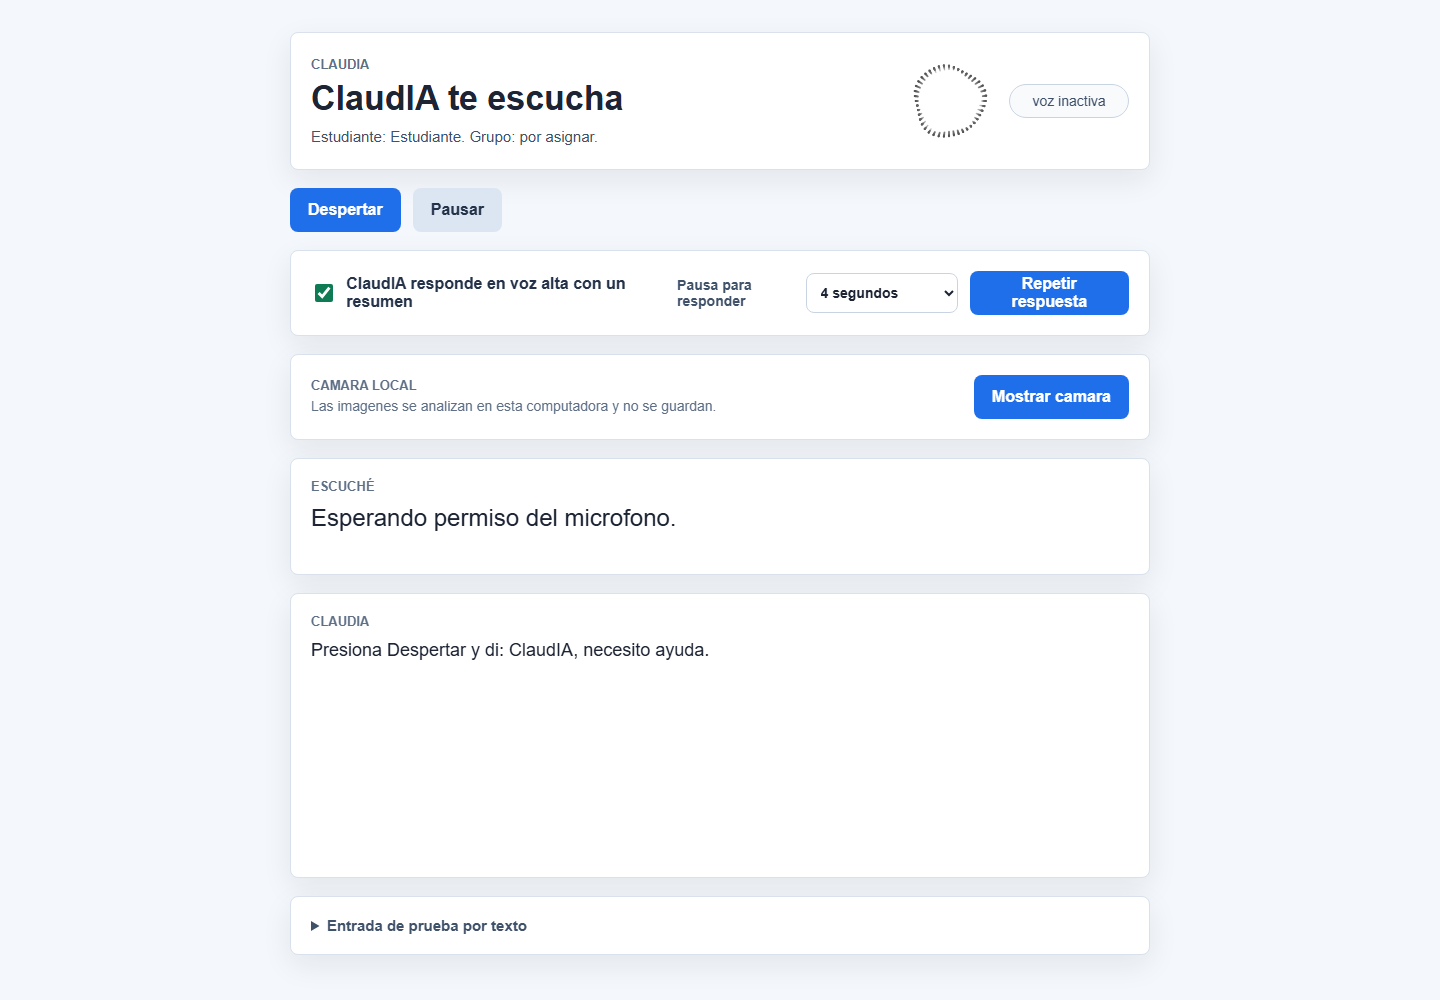
\includegraphics[width=5.12in,height=3.49in,keepaspectratio]{assets/interfaz_inicial.png}
\end{center}

\vspace{-0.17in}
\begin{tabularx}{\textwidth}{@{}>{\bfseries}p{1.45in}X@{}}
\toprule
Proyecto & ClaudIA: Sistema Inteligente de Acompañamiento Didáctico para Grupos DGETI \\
Código & 26-AT625 \\
Manual & Instalación, versión 2.0 \\
Entorno & Estación local para Windows, macOS o Linux \\
Plantel & CETis 20, Ciudad del Carmen, Campeche \\
Subsistema & DGETI-SEMS-SEP \\
\bottomrule
\end{tabularx}

\clearpage
\pagenumbering{arabic}
\setcounter{page}{1}

% Página 2
\begin{center}{\normalfont\fontsize{14}{17}\selectfont Índice}\end{center}
\vspace{20pt}
{\fontsize{11}{15.7}\selectfont
\TOCMain{1. Introducción}{sec:1}
\TOCMain{2. Objetivo del manual}{sec:2}
\TOCMain{3. Descripción general del sistema}{sec:3}
\TOCSub{3.1 Elementos que se instalan}
\TOCMain{4. Requisitos del sistema}{sec:4}
\TOCSub{4.1 Hardware y software}
\TOCSub{4.2 Servicios externos}
\TOCMain{5. Tecnologías utilizadas}{sec:5}
\TOCMain{6. Arquitectura del sistema}{sec:6}
\TOCMain{7. Instalación del entorno}{sec:7}
\TOCMain{8. Configuración de servicios}{sec:8}
\TOCMain{9. Variables de entorno}{sec:9}
\TOCMain{10. Estructura del proyecto}{sec:10}
\TOCMain{11. Ejecución del sistema}{sec:11}
\TOCMain{12. Pruebas de funcionamiento}{sec:12}
\TOCMain{13. Solución de errores comunes}{sec:13}
\TOCMain{14. Mantenimiento básico}{sec:14}
\TOCMain{15. Escalabilidad futura}{sec:15}
\TOCMain{16. Conclusiones}{sec:16}
\TOCMain{17. Anexos}{sec:17}
}

\clearpage
% Página 3
\SectionNum{1}{Introducción}
ClaudIA es una estación local de acompañamiento didáctico para estudiantes y docentes de grupos DGETI. La entrada principal es la voz y la salida puede reproducirse por bocina o mostrarse en pantalla. La cámara, cuando está disponible, detecta presencia o contexto general sin identificar personas.

Este manual describe la instalación técnica de una copia funcional. No requiere un servidor central: el navegador, Node.js y los archivos del repositorio se ejecutan en la misma computadora. Los servicios de inteligencia artificial se usan sólo cuando existe conexión y una clave configurada.

El sistema conserva un alcance educativo. No sustituye al docente, no califica automáticamente, no diagnostica condiciones de salud y no lee cuadernos para resolver ejercicios.

La instalación propuesta permite:
\begin{enumerate}
  \item Ejecutar la interfaz web local.
  \item Procesar voz y texto.
  \item Mantener contexto de estudiante y grupo.
  \item Utilizar el tutor, documentos y presentaciones.
  \item Activar la cámara local cuando sea necesaria.
\end{enumerate}

\clearpage
% Página 4
\SectionNum{2}{Objetivo del manual}
El objetivo es documentar una instalación reproducible de ClaudIA, desde la preparación del equipo hasta la verificación funcional.

El procedimiento permite:
\begin{enumerate}
  \item Instalar Node.js y las dependencias.
  \item Configurar DeepSeek como proveedor principal.
  \item Preparar la cámara y la generación de presentaciones como funciones opcionales.
  \item Ejecutar la interfaz local.
  \item Verificar el sistema mediante comandos y pruebas automatizadas.
  \item Mantener las claves y los datos locales fuera del repositorio.
\end{enumerate}

\SectionNum{3}{Descripción general del sistema}
ClaudIA funciona en una computadora del plantel. El usuario abre la interfaz en un navegador local, habla o escribe una consulta y recibe una respuesta visual y auditiva. El núcleo identifica si la entrada corresponde a un comando, una duda o una solicitud de práctica.

La estación no expone el servicio fuera de la computadora por configuración predeterminada. Tampoco requiere una base de datos central ni una aplicación instalada en el teléfono del estudiante.

\clearpage
% Página 5
\TableTitle{Funcionalidades principales}
\begin{enumerate}
  \item Interacción por voz y texto.
  \item Explicaciones graduales y preguntas de práctica.
  \item Contexto separado por estudiante y grupo.
  \item Lecciones, progreso y memoria local.
  \item Modo docente y preparación de clases.
  \item Detección local de presencia.
  \item Generación de presentaciones en PDF.
  \item Registro local de interacciones.
\end{enumerate}

\TableTitle{Usuarios y funciones}
\begin{center}
\renewcommand{\arraystretch}{1.18}
\begin{tabularx}{0.92\linewidth}{|>{\raggedright\arraybackslash}p{0.28\linewidth}|X|}
\hline
\rowcolor{tablehead}\textbf{Usuario} & \textbf{Función principal}\\
\hline
Estudiante & Formula consultas y realiza práctica guiada\\
\hline
Docente & Prepara clases, revisa temas y genera apoyos\\
\hline
Administrador & Instala, configura, actualiza y respalda\\
\hline
\end{tabularx}
\end{center}

\SubsectionNum{3.1}{Elementos que se instalan}
\begin{enumerate}
  \item Navegador Chrome o Edge.
  \item Node.js 20 o superior.
  \item Dependencias del proyecto.
  \item Archivo local de configuración.
  \item Python y OpenCV, opcionales para cámara.
  \item Compilador LaTeX, opcional para presentaciones.
\end{enumerate}

\clearpage
% Página 6
\SectionNum{4}{Requisitos del sistema}
\SubsectionNum{4.1}{Requisitos de hardware}
\begin{center}
\renewcommand{\arraystretch}{1.18}
\begin{tabularx}{0.92\linewidth}{|>{\raggedright\arraybackslash}p{0.34\linewidth}|X|}
\hline
\rowcolor{tablehead}\textbf{Componente} & \textbf{Requisito mínimo}\\
\hline
Procesador & Doble núcleo de 64 bits\\
\hline
Memoria RAM & 4 GB, 8 GB recomendados\\
\hline
Almacenamiento & 10 GB libres\\
\hline
Pantalla & 1366 x 768\\
\hline
Audio & Micrófono y bocina funcionales\\
\hline
Cámara & Opcional, con permiso local\\
\hline
Conectividad & Internet para respuestas de IA\\
\hline
\end{tabularx}
\end{center}

\SubsectionNum{4.2}{Requisitos de software}
\begin{itemize}
  \item Node.js 20 o superior.
  \item npm incluido con Node.js.
  \item Chrome o Edge actualizado.
  \item Git para obtener y actualizar el repositorio.
  \item Visual Studio Code, opcional para mantenimiento.
  \item Python 3 y OpenCV para la cámara.
  \item MiKTeX o TeX Live para presentaciones.
\end{itemize}

\clearpage
% Página 7
\SubsectionNum{4.3}{Servicios externos}
El tutor requiere un proveedor de lenguaje. DeepSeek es el proveedor principal predeterminado; OpenAI puede configurarse como respaldo.

\begin{center}
\begin{tabularx}{0.92\linewidth}{|>{\raggedright\arraybackslash}p{0.30\linewidth}|X|}
\hline
\rowcolor{tablehead}\textbf{Servicio} & \textbf{Uso}\\
\hline
DeepSeek API & Explicaciones y generación educativa\\
\hline
OpenAI API & Respaldo opcional\\
\hline
\end{tabularx}
\end{center}

\SubsectionNum{4.4}{Requisitos previos de configuración}
\begin{enumerate}
  \item Copia local del repositorio ClaudIA.
  \item Clave de DeepSeek o, en su defecto, de OpenAI.
  \item Permiso para ejecutar procesos locales.
  \item Micrófono y bocina configurados.
  \item Acceso a Internet durante las pruebas de IA.
\end{enumerate}

\SubsectionNum{4.5}{Consideraciones de conectividad}
La interfaz y los comandos locales pueden funcionar sin una clave de IA. Las explicaciones generativas no estarán disponibles hasta configurar un proveedor. Si la red falla durante una sesión, ClaudIA debe informar el problema y conservar el contexto general.

\clearpage
% Página 8
\SectionNum{5}{Tecnologías utilizadas}
\begin{center}
\renewcommand{\arraystretch}{1.18}
\begin{tabularx}{0.92\linewidth}{|>{\raggedright\arraybackslash}p{0.30\linewidth}|X|}
\hline
\rowcolor{tablehead}\textbf{Tecnología} & \textbf{Función}\\
\hline
Node.js & Ejecución del núcleo y servidor local\\
\hline
JavaScript & Lenguaje del sistema\\
\hline
Express & Servidor HTTP de la interfaz\\
\hline
OpenAI SDK & Cliente para DeepSeek y OpenAI\\
\hline
dotenv & Variables de entorno\\
\hline
Web Speech API & Voz en Chrome o Edge\\
\hline
Python y OpenCV & Detección local de presencia\\
\hline
LaTeX y MiKTeX & Presentaciones educativas\\
\hline
Git & Control de versiones\\
\hline
\end{tabularx}
\end{center}

\TableTitle{Justificación técnica}
Node.js permite integrar la interfaz web, el procesamiento de comandos y las llamadas a servicios de IA en un solo proceso local. Python queda aislado para visión. La generación de presentaciones usa una plantilla LaTeX controlada.

\clearpage
% Página 9
\SectionNum{6}{Arquitectura del sistema}
La arquitectura separa interfaz, núcleo, comandos, memoria, educación, tutoría, documentos, voz y visión. Esa división permite sustituir un componente sin reescribir el resto.

\begin{center}
\resizebox{0.85\textwidth}{!}{%
\begin{tikzpicture}[
  node distance=6mm,
  box/.style={draw,minimum width=3.4in,minimum height=0.34in,align=center},
  arr/.style={-{Latex[length=1.8mm]},line width=0.5pt}
]
\node[box] (browser) {Navegador: voz, texto y estado};
\node[box,below=of browser] (web) {WebVoiceInterface: servidor local};
\node[box,below=of web] (core) {Núcleo ClaudIA: eventos, comandos y sesión};
\node[box,below=of core] (edu) {Tutor, educación y memoria};
\node[box,below=of edu] (services) {DeepSeek / OpenAI / documentos / presentaciones};
\node[box,below=of services] (local) {Python, OpenCV, archivos y registros locales};
\foreach \a/\b in {browser/web,web/core,core/edu,edu/services,services/local}{\draw[arr](\a)--(\b);}
\end{tikzpicture}
}
\end{center}

\SubsectionNum{6.1}{Flujo general}
El navegador envía texto o una transcripción. La interfaz la convierte en un evento, el núcleo identifica la intención y el módulo correspondiente prepara la respuesta. La salida se muestra en pantalla y puede reproducirse por voz.

\clearpage
% Página 10
\SubsectionNum{6.2}{Componentes principales}
\begin{center}
\begin{tabularx}{0.94\linewidth}{|>{\raggedright\arraybackslash}p{0.30\linewidth}|X|}
\hline
\rowcolor{tablehead}\textbf{Componente} & \textbf{Función}\\
\hline
Interfaz web & Voz, texto, cámara y respuesta\\
\hline
Núcleo & Eventos, estado y ruteo\\
\hline
Comandos & Interpretan intenciones y ejecutan acciones\\
\hline
Educación y tutor & Lecciones, práctica y retroalimentación\\
\hline
Memoria & Sesión y persistencia por estudiante y grupo\\
\hline
Proveedor de IA & Genera explicaciones contextuales\\
\hline
Visión & Analiza presencia sin identificar personas\\
\hline
Presentaciones & Genera material visual en PDF\\
\hline
\end{tabularx}
\end{center}

\SubsectionNum{6.3}{Comunicación y seguridad}
La interfaz se enlaza con \texttt{127.0.0.1:3000}. Las solicitudes al proveedor de IA usan HTTPS. Las claves se cargan desde variables de entorno y no se incluyen en Git. La cámara procesa imágenes en la computadora y no conserva video por defecto.

\clearpage
% Página 11
\SectionNum{7}{Instalación del entorno}
\SubsectionNum{7.1}{Instalación de Node.js}
Descargue Node.js 20 o superior desde el sitio oficial. Instale la versión LTS y verifique desde PowerShell:
\begin{lstlisting}
node -v
npm -v
\end{lstlisting}
Ambos comandos deben mostrar una versión válida.

\SubsectionNum{7.2}{Obtención del proyecto}
Clone el repositorio o copie la carpeta completa en una ubicación local:
\begin{lstlisting}
git clone <URL_DEL_REPOSITORIO>
cd ClaudIA-repo
\end{lstlisting}

\SubsectionNum{7.3}{Instalación de dependencias}
\begin{lstlisting}
npm install
npm run setup
\end{lstlisting}
\texttt{npm install} instala los módulos. \texttt{npm run setup} crea el archivo local de configuración sin sobrescribir uno existente.

\clearpage
% Página 12
\SubsectionNum{7.4}{Verificación inicial}
Ejecute:
\begin{lstlisting}
npm run doctor
\end{lstlisting}
El diagnóstico debe confirmar:
\begin{itemize}
  \item Versión compatible de Node.js.
  \item Archivo \texttt{.env} disponible.
  \item Clave de IA configurada.
  \item Servicio local en \texttt{127.0.0.1}.
\end{itemize}

\SubsectionNum{7.5}{Dependencias opcionales}
\TableTitle{Cámara local}
\begin{lstlisting}
python -m pip install "opencv-python>=4.10.0"
\end{lstlisting}
\TableTitle{Presentaciones}
Instale MiKTeX o TeX Live y compruebe:
\begin{lstlisting}
pdflatex --version
\end{lstlisting}
Estas funciones pueden omitirse. Sin ellas, voz, texto y tutoría continúan disponibles.

\clearpage
% Página 13
\SectionNum{8}{Configuración de servicios}
\SubsectionNum{8.1}{Proveedor principal}
Abra el archivo \texttt{.env} y configure DeepSeek:
\begin{lstlisting}
AI_PROVIDER=deepseek
DEEPSEEK_API_KEY=tu_clave_local
DEEPSEEK_MODEL=deepseek-chat
DEEPSEEK_BASE_URL=https://api.deepseek.com
\end{lstlisting}
La clave debe obtenerse desde la cuenta autorizada del proyecto. No escriba la clave en el informe, la conversación ni el repositorio.

\SubsectionNum{8.2}{Proveedor de respaldo}
OpenAI es opcional:
\begin{lstlisting}
AI_FALLBACK_PROVIDER=openai
OPENAI_API_KEY=
OPENAI_MODEL=gpt-4.1-mini
\end{lstlisting}
Si DeepSeek no está disponible y existe respaldo, ClaudIA intentará continuar con el segundo proveedor.

\SubsectionNum{8.3}{Verificación del proveedor}
El comando \texttt{npm run doctor} informa el proveedor configurado. En la interfaz, una respuesta de tutor confirma que la clave y la conexión funcionan.

\clearpage
% Página 14
\SectionNum{9}{Variables de entorno}
El archivo \texttt{.env} se crea en la raíz del proyecto y permanece fuera de Git.

\begin{center}
\renewcommand{\arraystretch}{1.16}
\begin{tabularx}{\textwidth}{|>{\ttfamily}p{2.10in}|X|}
\hline
\rowcolor{tablehead}\normalfont\textbf{Variable} & \textbf{Función}\\
\hline
AI\_PROVIDER & Proveedor principal de IA\\
\hline
AI\_FALLBACK\_PROVIDER & Proveedor alternativo\\
\hline
DEEPSEEK\_API\_KEY & Credencial de DeepSeek\\
\hline
DEEPSEEK\_MODEL & Modelo de DeepSeek\\
\hline
OPENAI\_API\_KEY & Credencial opcional de OpenAI\\
\hline
VOICE\_HOST & Dirección local de la interfaz\\
\hline
VOICE\_PORT & Puerto de la interfaz\\
\hline
PYTHON\_COMMAND & Comando para visión\\
\hline
CAMERA\_INDEX & Cámara que se utilizará\\
\hline
\end{tabularx}
\end{center}

\TableTitle{Seguridad}
\begin{itemize}
  \item No comparta \texttt{.env}.
  \item Excluya claves y credenciales de Git.
  \item Mantenga \texttt{VOICE\_HOST=127.0.0.1}.
  \item Cambie la clave si se expone accidentalmente.
\end{itemize}

\clearpage
% Página 15
\SectionNum{10}{Estructura del proyecto}
\begin{lstlisting}
ClaudIA-repo/
|-- src/
|   |-- ai/            proveedores y prompts
|   |-- bootstrap/     composición del sistema
|   |-- classroom/     contexto docente
|   |-- commands/      intérpretes y acciones
|   |-- config/        perfil y variables
|   |-- core/          eventos, estado y comandos
|   |-- documents/     lectura local
|   |-- education/     lecciones y progreso
|   |-- interface/     terminal y web
|   |-- logs/          registro local
|   |-- memory/        sesión y persistencia
|   |-- presentations/ generación LaTeX
|   |-- tutor/         acompañamiento didáctico
|   |-- vision/        Python y OpenCV
|   `-- voice/         procesamiento de voz
|-- tests/             pruebas automatizadas
|-- docs/              documentación técnica
|-- scripts/           instalación y diagnóstico
|-- .env.example       configuración de referencia
`-- package.json       dependencias y comandos npm
\end{lstlisting}

\clearpage
% Página 16
\TableTitle{Responsabilidad de las carpetas}
\begin{center}
\begin{tabularx}{0.94\linewidth}{|>{\ttfamily}p{1.55in}|X|}
\hline
\rowcolor{tablehead}\normalfont\textbf{Carpeta} & \textbf{Uso}\\
\hline
src/core & Núcleo, eventos y estado\\
\hline
src/commands & Interpretación y ejecución\\
\hline
src/education & Lecciones y progreso\\
\hline
src/tutor & Preguntas, pistas y práctica\\
\hline
src/interface & Terminal y aplicación web\\
\hline
src/vision & Detección local de presencia\\
\hline
src/presentations & Generación y compilación\\
\hline
tests & Pruebas del sistema\\
\hline
\end{tabularx}
\end{center}

\SubsectionNum{10.1}{Archivos que no deben versionarse}
\texttt{node\_modules/}, \texttt{.env}, \texttt{data/}, \texttt{generated/} y los archivos de registro quedan fuera del repositorio. Al restaurar una instalación deben crearse de nuevo mediante los comandos del proyecto.

% Página 17
\SectionNum{11}{Ejecución del sistema}
Desde la raíz del proyecto:
\begin{lstlisting}
npm start
\end{lstlisting}
Después abra:
\begin{center}\texttt{http://127.0.0.1:3000}\end{center}

La variante de terminal se inicia con:
\begin{lstlisting}
npm run terminal
\end{lstlisting}

\SectionNum{12}{Pruebas de funcionamiento}
Ejecute la batería completa:
\begin{lstlisting}
npm test
\end{lstlisting}
La versión documentada contiene 92 pruebas aprobadas.

\clearpage
\TableTitle{Comprobación funcional}
\begin{enumerate}
  \item La interfaz abre en el navegador.
  \item El comando \texttt{ayuda} responde.
  \item El estudiante y el grupo se muestran correctamente.
  \item La voz recibe la transcripción y produce una respuesta.
  \item La entrada por texto funciona como alternativa.
  \item La cámara informa su disponibilidad sin bloquear el tutor.
\end{enumerate}

\begin{center}
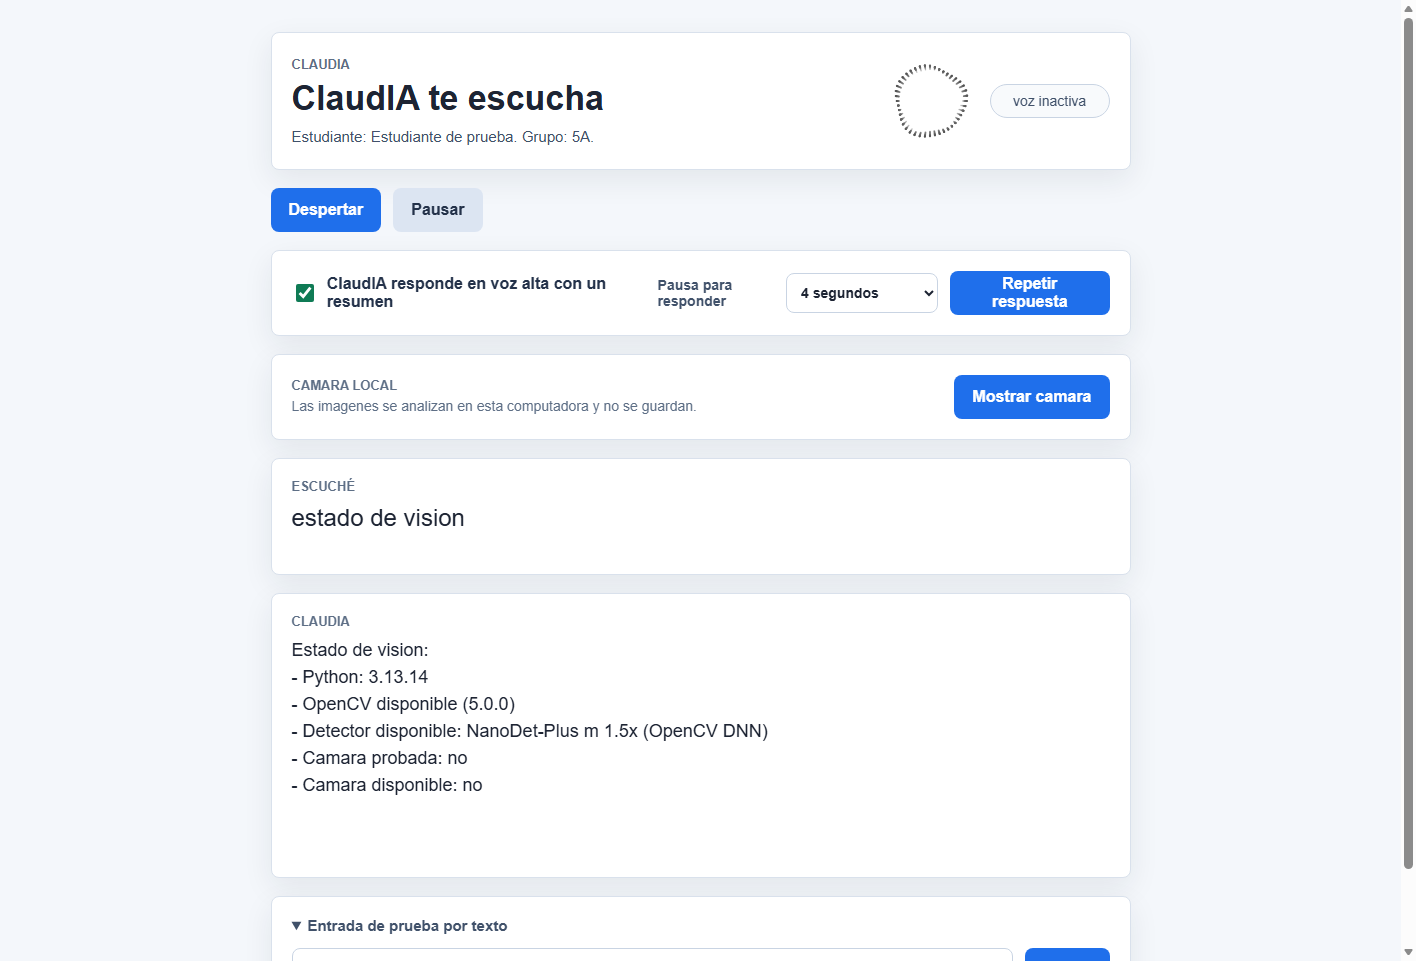
\includegraphics[width=3.70in,height=2.45in,keepaspectratio]{assets/estado_vision.png}
\end{center}

\FigureCaption{Figura 1: Diagnóstico de visión y disponibilidad de la cámara.}

\clearpage
% Página 18
\SectionNum{13}{Solución de errores comunes}
\TableTitle{Errores de instalación}
\begin{center}
\renewcommand{\arraystretch}{1.16}
\begin{tabularx}{\textwidth}{|>{\raggedright\arraybackslash}p{1.55in}|X|}
\hline
\rowcolor{tablehead}\textbf{Mensaje o síntoma} & \textbf{Comprobación}\\
\hline
Node.js no reconocido & Reinstale la versión LTS y abra una terminal nueva\\
\hline
Puerto 3000 ocupado & Cambie \texttt{VOICE\_PORT} o cierre el proceso anterior\\
\hline
Falta DEEPSEEK\_API\_KEY & Edite \texttt{.env} y ejecute \texttt{npm run doctor}\\
\hline
Micrófono bloqueado & Revise el permiso del sitio en Chrome o Edge\\
\hline
OpenCV no disponible & Instale OpenCV o desactive la cámara\\
\hline
No se genera PDF & Verifique MiKTeX y el comando \texttt{pdflatex}\\
\hline
Respuesta de IA vacía & Revise conexión, clave y proveedor configurado\\
\hline
\end{tabularx}
\end{center}

\SectionNum{14}{Mantenimiento básico}
\begin{enumerate}
  \item Ejecute \texttt{npm test} después de cada actualización.
  \item Revise \texttt{npm run doctor} antes de una sesión.
  \item Actualice dependencias con revisión previa.
  \item Respalde \texttt{.env} en un medio seguro.
  \item Verifique audio y cámara semanalmente.
  \item Elimine datos de prueba al terminar el ciclo.
\end{enumerate}

\clearpage
% Página 19
\SectionNum{15}{Escalabilidad futura}
La instalación puede crecer en cuatro direcciones:
\begin{enumerate}
  \item Agregar una presentación institucional más clara de la interfaz.
  \item Incorporar adaptadores para micrófono, bocina y carcasa.
  \item Ampliar el catálogo de lecciones por asignatura.
  \item Evaluar un panel docente con mayor capacidad de agregación.
\end{enumerate}

Estas mejoras deben conservar el procesamiento local, la separación de módulos y la posibilidad de operar sin un servidor central.

\SectionNum{16}{Conclusiones}
ClaudIA puede instalarse en una computadora del plantel con Node.js, un navegador compatible y una clave de IA. La voz, el texto y los comandos están disponibles desde la misma interfaz.

La cámara y las presentaciones son componentes opcionales. Su ausencia no impide utilizar el tutor ni ejecutar las pruebas principales. Antes de trasladar la estación al aula, deben completarse el diagnóstico, las pruebas y una sesión funcional supervisada.

\clearpage
% Página 20
\SectionNum{17}{Anexos}
\SubsectionNum{A}{Comandos de instalación}
\begin{lstlisting}
git clone <URL_DEL_REPOSITORIO>
cd ClaudIA-repo
npm install
npm run setup
npm run doctor
npm test
npm start
\end{lstlisting}

\SubsectionNum{B}{Comandos opcionales}
\begin{lstlisting}
python -m pip install "opencv-python>=4.10.0"
pdflatex --version
\end{lstlisting}

\SubsectionNum{C}{Lista de comprobación}
\begin{enumerate}
  \item Node.js 20 o superior.
  \item Dependencias instaladas.
  \item Archivo \texttt{.env} configurado.
  \item Clave de IA validada.
  \item Interfaz disponible en el puerto local.
  \item Micrófono y bocina comprobados.
  \item Pruebas automatizadas aprobadas.
\end{enumerate}

\SubsectionNum{D}{Datos del proyecto}
\begin{center}
\begin{tabularx}{\textwidth}{@{}>{\bfseries}p{1.45in}X@{}}
\toprule
Proyecto & ClaudIA: Sistema Inteligente de Acompañamiento Didáctico para Grupos DGETI \\
Código & 26-AT625 \\
Versión & 0.3.0 \\
Repositorio & \texttt{ClaudIA-repo} \\
Revisión & \texttt{29db70a} \\
Pruebas & 92 aprobadas \\
\bottomrule
\end{tabularx}
\end{center}

\end{document}
